\documentclass[11pt]{article}

% Wiley-style formatting for Journal of Software: Evolution and Process
\usepackage[margin=1in]{geometry}
\usepackage{times} % Wiley uses Times font

% Essential packages
\usepackage[numbers,sort&compress]{natbib}
\usepackage{amsmath,amssymb,amsfonts,amsthm}
\newtheorem{definition}{Definition}
\usepackage{algorithmic}
\usepackage{algorithm}
\usepackage{graphicx}
\usepackage{url}
\usepackage[english]{babel}
\usepackage[autostyle, english = american]{csquotes}
\MakeOuterQuote{"}

\usepackage{float}
\floatstyle{plain}
\newfloat{listing}{htbp}{lop}
\floatname{listing}{Listing}

\usepackage{multirow}
\usepackage{listings}
\usepackage{xcolor}
\usepackage{booktabs}
\usepackage{tikz}
\usetikzlibrary{shapes.geometric, arrows, positioning, fit, backgrounds}
\usepackage{pgfplots}
\pgfplotsset{compat=1.17}
\usepackage{subcaption}
\usepackage[colorlinks=true,linkcolor=blue,citecolor=blue,urlcolor=blue]{hyperref}
\usepackage{cleveref}

% Line numbers for review
\usepackage{lineno}

% Wiley-style section formatting
\usepackage{titlesec}
\titleformat{\section}{\large\bfseries}{\thesection}{1em}{}
\titleformat{\subsection}{\normalsize\bfseries}{\thesubsection}{1em}{}
\titleformat{\subsubsection}{\normalsize\itshape}{\thesubsubsection}{1em}{}

\definecolor{codegray}{rgb}{0.5,0.5,0.5}
\definecolor{codeblue}{rgb}{0.0,0.0,0.6}
\definecolor{codegreen}{rgb}{0,0.5,0}
\definecolor{lightblue}{RGB}{173,216,230}
\definecolor{lightgreen}{RGB}{144,238,144}
\definecolor{lightyellow}{RGB}{255,255,224}
\definecolor{lightpurple}{RGB}{221,160,221}

\lstdefinestyle{code}{
  language=Java,
  basicstyle=\fontsize{9}{11}\selectfont\ttfamily,
  numbers=none,
  numberstyle=\tiny\color{codegray},
  stepnumber=1,
  numbersep=5pt,
  backgroundcolor=\color{white},
  showspaces=false,
  showstringspaces=false,
  showtabs=false,
  frame=single,
  rulecolor=\color{black},
  tabsize=2,
  captionpos=b,
  breaklines=true,
  breakatwhitespace=true,
  title=\lstname,
  keywordstyle=\color{codeblue},
  commentstyle=\color{codegreen}\itshape,
  stringstyle=\color{red},
  escapeinside={(*@}{@*)},
  morekeywords={*,...}
}

\lstset{style=code}

\usepackage{textcomp}

% Running headers
\usepackage{fancyhdr}
\pagestyle{fancy}
\fancyhf{}
\fancyhead[L]{\small\itshape Edmonds and Utting}
\fancyhead[R]{\small\itshape J. Softw. Evol. Process}
\fancyfoot[C]{\thepage}
\renewcommand{\headrulewidth}{0.4pt}

\begin{document}

% Line numbers for peer review
\linenumbers

% Article type
\noindent\textbf{RESEARCH ARTICLE}
\vspace{1em}

% Title
\begin{center}
{\LARGE\bfseries Do Specifications Help LLMs Write Better Unit Tests?}
\vspace{1.5em}

% Authors
{\large Brendan Edmonds\textsuperscript{1}* \quad Mark Utting\textsuperscript{1}}
\vspace{0.5em}

% Affiliations
{\small\textsuperscript{1}UQ Cyber, School of Electrical Engineering and Computer Science, University of Queensland, St Lucia QLD 4067, Australia}
\vspace{0.5em}

% Correspondence
{\small *Correspondence: Brendan Edmonds, b.edmonds@uq.edu.au}
\end{center}

\vspace{1em}

% Abstract
\noindent\textbf{Abstract}
\vspace{0.5em}

\noindent Large language models can generate unit tests from method signatures, but the resulting tests are weakened by the absence of an oracle: signatures convey what a method takes and returns, not what it should do. This article asks whether giving the model a \emph{specification}---a precise statement of what the method should do---measurably improves the tests it produces, with quality assessed by mutation testing. The question is answered through a controlled four-phase comparison on 312 methods from Apache Commons Lang. The same model (Gemini~2.0, temperature 0.3, five independent runs per configuration) is given (P1)~the method signature alone, (P2)~the signature with edge-case guidance, (P3)~the signature together with a specification, and (P4)~the full method source code as an upper-bound baseline.

The answer is yes, and the effect is large. Specifications raise test count by 272\% and mutation score by 40.7~percentage points relative to signatures alone ($p < 0.001$, Cohen's $d = 2.41$). Specifications also raise the compilation rate from 89.2\% to 91.5\% and the pass rate from 94.1\% to 96.8\%, which suggests they constrain the model toward syntactically and semantically correct test code. Full source code (P4) attains the highest absolute scores (94.8\% mutation), but the specification phase closes most of the gap to source while remaining materially more compact.

To make the study tractable at 312 methods, the specifications are produced automatically by JML-Inferrer, a static analysis system developed alongside the experiment. JML-Inferrer infers JML method contracts using heuristic pattern matching organised by weakest-precondition and strongest-postcondition reasoning, and discharges each inferred clause through OpenJML's Extended Static Checker. On the same corpus, the system attains 94.2\%/89.3\% precision/recall for preconditions and 87.6\%/78.1\% for postconditions under two-rater manual validation. A complete replication package accompanies the article.

\vspace{1em}

% Keywords
\noindent\textbf{Keywords:} LLM-based test generation; mutation testing; specification inference; JML; oracle problem; large language models; static analysis

\vspace{1em}
\hrule
\vspace{1em}

\section{Introduction}
\label{sec:introduction}

Large language models (LLMs) have rapidly become a practical means of generating unit tests from source code~\cite{schafer2023adaptive, chen2022codet, yuan2024chattester, lemieux2023codamosa, chen2021codex}, and an extensive recent literature has emerged around the technique~\cite{zhang2025llmunitsurvey}. Given a method signature, a modern LLM produces compilable, plausibly named tests in seconds; given the source body, it produces tests that exercise visible control-flow paths. The persistent weakness, well documented across the field~\cite{schafer2023adaptive, jiang2024survey, konstantinou2024oracles}, is the \emph{oracle problem}: the generated tests assert what the implementation does, not what it should do. Konstantinou et al.~\cite{konstantinou2024oracles} show empirically that LLM-generated oracles tend to encode the program's actual behaviour rather than its intended behaviour; when the implementation is buggy the model dutifully encodes the bug as the expected behaviour, and when the model is given only a signature it has no oracle at all and falls back to weak assertions such as ``does not throw''.

Formal specifications are the classical answer to the oracle problem~\cite{meyer1992design, jml, leavens2006design}, but their adoption is limited by the cost of writing them~\cite{matichuk_cost_2015, hall1990seven, zimmermann2019lightweight}. The empirical question this article addresses is therefore practical rather than theoretical: \emph{does giving a specification to an LLM measurably improve the unit tests it writes?} The hypothesis is that a specification---even one that is heuristically derived and incomplete---carries oracle information that is absent from the signature and largely redundant with the source body, and that this information is dense enough to shift LLM-generated tests from coverage-driven artefacts toward genuine behavioural checks.

The test-generation question is the headline empirical question because it has a clean answer under mutation testing, but it is one of several downstream uses of the same inferred specifications. The first is stronger LLM test oracles, the focus of the present article. The second is \emph{compositional verification of calling code}: a verifier that needs the contract of a callee in order to reason about a caller currently has either to verify the whole transitive dependency graph or to require manual contracts at every library boundary; inferred specifications act as the callee summaries that the caller's verification condition needs, so a change to a library entry implies a check of the calls that depend on it rather than a re-analysis of the entire program. The third is \emph{agentic programming}: an AI coding agent asked to interact with a library that postdates its training cut-off has no internal model of that library's contracts, and the same JML annotations function as a machine-readable contract the agent can consume to ground its reasoning. Throughout this article the inference machinery is treated as serving all three uses; the empirical evaluation isolates the first one because it is the use whose effect size mutation testing can measure within the budget of a single study.

The hypothesis is tested by holding the model fixed and varying only the input given to it. Four conditions are compared on the same 312-method corpus drawn from Apache Commons Lang: \textbf{P1}, the method signature alone; \textbf{P2}, signature with explicit guidance to cover edge cases; \textbf{P3}, signature together with a specification; \textbf{P4}, the full method source code as an upper-bound baseline. Test quality is measured by test count, compilation rate, pass rate, and mutation score (PIT~\cite{coles2016pitest}). P2 is included precisely to address the alternative hypothesis that any explicit guidance, not specifications in particular, would suffice: it does not---P2 generates the most tests but attains a lower mutation score than~P3, showing that test count is a poor proxy for oracle strength.

The methodological challenge is that 312 specifications cannot be written by hand within the budget of a single study. They are therefore inferred automatically by JML-Inferrer, a static analysis system developed alongside this study and described in Section~\ref{sec:approach}. The Java Modeling Language~(JML)~\cite{jml,leavens2006design} provides the contract notation used throughout. The JML-Inferrer is the means by which the empirical question becomes answerable at scale.

We make the following contributions:

\begin{enumerate}
    \item An affirmative empirical answer to the title question, with effect size: specifications increase the LLM's test count by 272\% (95\% bootstrap CI~$[245, 299]$) and mutation score by 40.7~percentage points relative to signatures alone ($p < 0.001$, Cohen's $d = 2.41$, 95\% bootstrap CI~$[2.08, 2.79]$).

    \item A breakdown of the effect by method category and by mutation operator, identifying where specifications carry the most oracle information (control-flow and utility methods) and where signature-only generation is already near-optimal (simple accessors).

    \item JML-Inferrer, the static analysis system used to produce the specifications, organised by weakest-precondition and strongest-postcondition reasoning and validated against OpenJML's Extended Static Checker.

    \item A probe-and-backport development methodology that uses an LLM to draft candidate JML, OpenJML's Extended Static Checker to filter discharged from undischarged clauses, and an agentic coding assistant to extend the inference engine until the discharged examples are emitted automatically. The methodology is what produced the heuristic repertoire underlying the experimental results, and is offered both as an account of how the system was developed and as a recipe for users who need to extend it (Section~\ref{subsec:probe-backport}).

    \item A replication package containing the source code, datasets, inferred specifications, generated test suites, and analysis scripts.
\end{enumerate}

Apache Commons Lang is used as the evaluation subject because it provides a mature, well-documented codebase with diverse method implementations and is widely adopted in software-engineering research~\cite{pacheco2007randoop, fraser2011evosuite}. The findings reported here motivate a planned follow-up study on service-boundary code (REST clients, RPC stubs), where the oracle problem is most acute and the effect reported here is expected to compound. The two remaining use cases identified above---compositional verification of callers and agentic programming over post-cut-off libraries---are the subject of separate ongoing work on specification distribution and on the agent-consumable contract format, and are mentioned here only to indicate that the inference machinery is not test-generation-specific.

\section{Background: What Counts as a Specification}
\label{sec:background}

The central question of this article hinges on what is given to the LLM in phase P3---namely, a \emph{specification} of a method's intended behaviour in the form of pre- and postconditions. This section establishes what those specifications look like and which classical analyses justify them; the next section describes how they are produced automatically.

The two classical directions of program reasoning are complementary. Weakest-precondition (WP) analysis~\cite{dijkstra_guarded_1975, dijkstra1976discipline} computes, for a statement $S$ and postcondition $Q$, the weakest predicate $\text{WP}(S, Q)$ on the entry state under which every terminating execution of $S$ establishes $Q$. Strongest-postcondition (SP) analysis~\cite{hoare1969axiomatic, cousot1977abstract} computes, for a precondition $P$, the strongest predicate $\text{SP}(S, P)$ that holds on the exit state. WP propagates obligations backward from desired outcomes; SP propagates known facts forward from assumed inputs.

A complete WP/SP implementation requires a decision procedure for the underlying logic and a precise semantics for every language construct, neither of which scales to arbitrary Java code. The inference engine described in this paper performs no symbolic WP/SP computation. Instead, the WP and SP calculi are used as a \emph{design discipline}: they determine which abstract syntax tree (AST) patterns the engine recognises, what JML clause each pattern produces, and how clauses are propagated across procedure boundaries. The remainder of this section makes that mapping explicit; the corresponding implementation is described in Section~\ref{sec:approach}.

\subsection{Precondition Inference}
\label{subsec:wp-mapping}

Guard-and-throw idioms in Java methods correspond directly to WP obligations on the method entry state. Given a body in which an early statement \texttt{if (G) throw \dots} aborts execution, a WP analysis with $Q$ taken as the post of the normal-return path propagates $\neg G$ backward to the entry; the precondition is whatever must hold on entry to avoid the throw. JML-Inferrer recognises throw-, return-, and validation-style guards and emits the negation of each guard as a \texttt{requires} clause. Range checks of the form \texttt{if (i < 0 || i >= n) throw} yield two conjuncts; null guards yield non-nullness preconditions; chained dereferences contribute their definedness conditions ($\text{def}(e)$ in WP terminology --- non-null receiver, in-bounds index, non-zero divisor).

The same discipline determines what the engine deliberately omits. A condition controlling branching logic that does not abort, such as an \texttt{if/else} where both branches return a value, carries no WP obligation on the entry state and is therefore excluded from precondition inference. Subconditions of ternary expressions are treated identically. This filter prevents internal control flow from being misclassified as a contract requirement.

\subsection{Postcondition Inference}
\label{subsec:sp-mapping}

Postconditions are forward-flow facts derived from return statements and field assignments. Each return statement \texttt{return $e$} contributes the SP-derived clause $\texttt{\textbackslash result} = e$, and each field assignment \texttt{this.f = $e$} contributes $\texttt{this.f} = e$ evaluated in the pre-state. Substituting field references with $\texttt{\textbackslash old}(\cdot)$ in the right-hand side captures the SP convention that assignments refer to the prior state.

Branching is handled at finer granularity than the textbook SP rule for conditionals, which combines two branches via $\text{SP}(S_1, P \land C) \lor \text{SP}(S_2, P \land \neg C)$. Emitting that disjunction directly would discard the path information that links each return value to its enabling condition. Instead, returns are recorded with the path conditions that reach them, and the inferred specification contains independent guarded clauses $C \Rightarrow \texttt{post}_1$ and $\neg C \Rightarrow \texttt{post}_2$. Ternary expressions are decomposed into the same form. Path conditions are simplified algebraically before emission (for instance, $x \le 0 \land x < 0$ reduces to $x < 0$, and $x \le 0 \land x \ge 0$ reduces to $x = 0$) so that the resulting JML remains readable.

\subsection{Interprocedural Propagation}
\label{subsec:proc-summaries}

Method calls are handled through procedure summaries, the standard mechanism for modular WP/SP analysis. Methods are analysed in dependency order during a first pass, and their inferred specifications are cached. When inference subsequently encounters a call site $\texttt{m}(a_1, \ldots, a_k)$, the cached pre- and post-conditions of \texttt{m} are instantiated by formal-to-actual parameter substitution, exactly as a textbook WP rule for procedure call would prescribe. Calls into the Java standard library are resolved against a curated specification database covering common operations on \texttt{String}, \texttt{Math}, \texttt{List}, \texttt{Map}, and utility classes; calls into other unannotated methods are treated as uninterpreted, with conservative summaries that may throw, may modify accessible state, and return unconstrained values.

\subsection{Loop Invariants}
\label{subsec:loop-mapping}

Loops are the principal site at which WP/SP reasoning is incomplete by syntax alone: the rule for $\text{WP}(\text{while } C \text{ do } S, Q)$ requires a loop invariant, which no purely syntactic procedure can derive. JML-Inferrer addresses this obligation through four complementary heuristics: bound-based invariants for counter loops, accumulator pattern detection, monotonicity inference from update expressions, and bounded symbolic unrolling (three iterations) as a fallback. Quantified loop invariants that remain valid at loop termination are promoted to method postconditions by substituting the loop counter with its exit value, allowing established loop facts to flow into the SP of the surrounding method. When all four heuristics fail to derive a non-trivial invariant, a conservative weak invariant is emitted in preference to nothing, so that the WP obligation is at least partially discharged.

\subsection{Parameter Treatment}
\label{subsec:parameter-handling}

Java parameters are mutable, which would render postconditions ambiguous in the presence of re-assignment. Following the standard SP convention, each parameter \texttt{x} is modelled as a fresh entry-value variable, and postconditions are expressed in terms of that entry value. In emitted JML this convention is rendered using the original parameter name (which JML interprets as the entry value) for parameters and \texttt{\textbackslash old(\dots)} for fields.

\subsection{Soundness Recovery via Formal Validation}
\label{subsec:soundness-recovery}

Because the engine matches AST patterns rather than performing symbolic computation, individual clauses are not guaranteed sound by construction; the WP/SP framing prescribes \emph{what} the engine looks for, not whether each emitted clause is provable. Soundness is recovered \emph{a posteriori} by discharging every emitted clause through OpenJML's Extended Static Checker~\cite{openjml} (Section~\ref{subsec:validation}). Clauses that fail verification are flagged for review rather than silently retained, and a regression test suite of 576 end-to-end verification tests gates the inference engine against this oracle. The empirical question of how closely the heuristic engine approximates a complete WP/SP analysis is addressed in Section~\ref{sec:results}.

\section{The Inference Instrument}
\label{sec:approach}

The empirical study in Section~\ref{sec:results} requires specifications to be available for every method in the corpus. Since manual specification at that scale is infeasible, the study is enabled by JML-Inferrer, a static analysis system developed alongside the experiment (Figure~\ref{fig:architecture}). This section describes JML-Inferrer at the level of detail required to interpret the empirical results; full implementation details, algorithm pseudocode, and the standard library specification database are provided in the Supplementary Material (Appendix~A--C).

\begin{figure}[t]
\centering
\resizebox{\textwidth}{!}{%
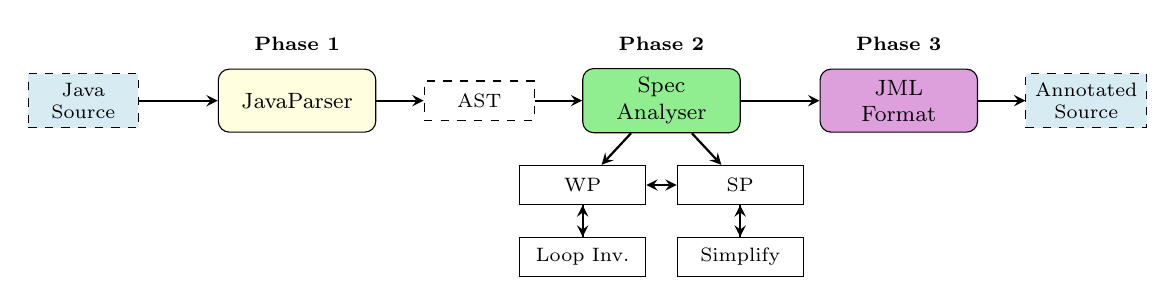
\begin{tikzpicture}[
    node distance=0.6cm and 0.8cm,
    component/.style={rectangle, draw, rounded corners, minimum width=2cm, minimum height=0.8cm, align=center, font=\footnotesize},
    subcomponent/.style={rectangle, draw, minimum width=1.6cm, minimum height=0.5cm, align=center, font=\scriptsize},
    data/.style={rectangle, draw, dashed, minimum width=1.4cm, minimum height=0.5cm, align=center, font=\scriptsize},
    arrow/.style={->, >=stealth, thick},
    phase/.style={rectangle, draw=gray, dashed, rounded corners, inner sep=0.2cm}
]

    % Input
    \node[data, fill=lightblue!50] (input) {Java\\Source};

    % Phase 1: Parsing
    \node[component, fill=lightyellow, right=1cm of input] (parser) {JavaParser};
    \node[data, right=0.6cm of parser] (ast) {AST};

    % Phase 2: Analysis
    \node[component, fill=lightgreen, right=0.6cm of ast] (analyzer) {Spec\\Analyser};

    % Sub-components of analyzer (below)
    \node[subcomponent, below=0.4cm of analyzer, xshift=-1cm] (wp) {WP};
    \node[subcomponent, below=0.4cm of analyzer, xshift=1cm] (sp) {SP};
    \node[subcomponent, below=0.4cm of wp] (loop) {Loop Inv.};
    \node[subcomponent, below=0.4cm of sp] (simp) {Simplify};

    % Phase 3: Output
    \node[component, fill=lightpurple, right=1cm of analyzer] (formatter) {JML\\Format};
    \node[data, fill=lightblue!50, right=0.6cm of formatter] (output) {Annotated\\Source};

    % Arrows - main flow
    \draw[arrow] (input) -- (parser);
    \draw[arrow] (parser) -- (ast);
    \draw[arrow] (ast) -- (analyzer);
    \draw[arrow] (analyzer) -- (formatter);
    \draw[arrow] (formatter) -- (output);

    % Arrows - subcomponents
    \draw[arrow] (analyzer) -- (wp);
    \draw[arrow] (analyzer) -- (sp);
    \draw[arrow] (wp) -- (loop);
    \draw[arrow] (sp) -- (simp);
    \draw[arrow, <->] (wp) -- (sp);
    \draw[arrow] (loop) -- (wp);
    \draw[arrow] (simp) -- (sp);

    % Phase labels
    \node[above=0.1cm of parser, font=\scriptsize\bfseries] {Phase 1};
    \node[above=0.1cm of analyzer, font=\scriptsize\bfseries] {Phase 2};
    \node[above=0.1cm of formatter, font=\scriptsize\bfseries] {Phase 3};

\end{tikzpicture}%
}
\caption{System architecture. Phase~1 parses Java source into an AST. Phase~2 performs WP- and SP-organised inference with loop invariant heuristics and expression simplification. Phase~3 emits inferred specifications as JML annotations.}
\label{fig:architecture}
\end{figure}

JML-Inferrer is implemented in Java~21 (approximately 20{,}000 lines of code at the time of submission) and uses JavaParser~\cite{javaparser} for AST construction. The pipeline comprises three phases: parsing, specification inference, and formatting. Source files are processed recursively, with annotations inserted in place, at an average of 88\,ms per file. The system is released under the Apache License 2.0; the present section describes only Phase~2, which contains the core inference logic. Phase~1 and Phase~3 are standard.

\subsection{Specification Inference}

The inference engine applies the visitor pattern over AST nodes, with pattern matching organised by the WP/SP correspondences described in Section~\ref{sec:background}. Symbolic execution~\cite{king1976symbolic, cadar2008klee} and full WP/SP computation are avoided deliberately; both require an SMT decision procedure and a complete operational semantics for Java, neither of which scales to arbitrary code. Pattern matching trades formal completeness for scalability and broad applicability, an established trade-off in industrial static analysis~\cite{calcagno2015infer}. Algorithm~\ref{alg:inference} sets out the inference procedure; the paragraphs that follow describe its principal components.

\begin{algorithm}[t]
\caption{Specification Inference via Pattern Matching}
\label{alg:inference}
\begin{algorithmic}[1]
\REQUIRE Method AST node $M$
\ENSURE Preconditions $Pre$, Postconditions $Post$, LoopInvariants $LI$
\STATE $Pre \gets \emptyset$; $Post \gets \emptyset$; $LI \gets \emptyset$
\STATE \COMMENT{Infer preconditions from early guards}
\FOR{each statement $S$ in $M$.body}
    \IF{$S$ is null check \texttt{if (p == null) throw/return}}
        \STATE $Pre \gets Pre \cup \{\texttt{p != null}\}$
    \ELSIF{$S$ is range check \texttt{if (p < 0 || p >= n) throw}}
        \STATE $Pre \gets Pre \cup \{\texttt{p >= 0}, \texttt{p < n}\}$
    \ENDIF
\ENDFOR
\STATE \COMMENT{Infer postconditions from return statements}
\FOR{each \texttt{return $e$} in $M$.body}
    \IF{$e$ is field access \texttt{this.f}}
        \STATE $Post \gets Post \cup \{\texttt{\textbackslash result == this.f}\}$
    \ELSIF{$e$ is new object \texttt{new T(...)}}
        \STATE $Post \gets Post \cup \{\texttt{\textbackslash result != null}\}$
    \ELSIF{$e$ involves \texttt{\textbackslash old} pattern}
        \STATE $Post \gets Post \cup \{$derive relationship$\}$
    \ENDIF
\ENDFOR
\STATE \COMMENT{Infer branch-conditional postconditions via symbolic paths}
\FOR{each return $r$ reached under path condition $\pi$ (if/else or ternary)}
    \STATE simplify $\pi$ algebraically
    \STATE $Post \gets Post \cup \{\pi \Longrightarrow \text{spec}(r)\}$
\ENDFOR
\FOR{each conditional field assignment \texttt{this.f = $e$} under path $\pi$}
    \STATE $Post \gets Post \cup \{\pi \Longrightarrow \mathtt{this.f} == e[\backslash\mathit{old}/\cdot]\}$
\ENDFOR
\STATE \COMMENT{Infer loop invariants}
\FOR{each loop $L$ in $M$.body}
    \STATE $LI \gets LI \cup \text{InferLoopInvariant}(L)$
\ENDFOR
\RETURN $(Pre, Post, LI)$
\end{algorithmic}
\end{algorithm}

\paragraph{Loops, procedure summaries, and branching.}
Loop invariant inference proceeds through four complementary heuristics: bound-based invariants for counter loops, accumulator pattern detection, monotonicity inference from update expressions, and bounded symbolic unrolling as a fallback. When all four fail, a conservative weak invariant is emitted. Across the 68 loops in 48 methods of the evaluation corpus, the non-trivial-invariant rate was 85.3\%; the four heuristics apply uniformly to \texttt{for}, \texttt{while}, and \texttt{for-each} constructs (Supplementary Material, Appendix~B).

Method calls are handled in two passes. The first analyses methods in dependency order and caches the inferred specification of each; the second propagates these specifications across call sites. Calls into unannotated methods are treated as uninterpreted (the callee may throw, may modify accessible state, and returns an unconstrained value). Calls into the Java standard library are resolved against a curated specification database covering common operations on \texttt{String}, \texttt{Math}, \texttt{List}, \texttt{Map}, and utility classes (Supplementary Material, Appendix~C).

A lightweight symbolic executor records a \emph{path condition} for each return statement, enabling branch-conditional postconditions of the form $\texttt{cond} \Longrightarrow \texttt{post}$. Both \texttt{if}/\texttt{else} and ternary branches are decomposed into per-path symbolic returns rather than collapsed into disjunctions, preserving the link between each return value and its enabling condition. Path conditions are simplified algebraically before emission. Heuristics that would be unsound under Java's two's-complement integer semantics (for instance, $\texttt{\textbackslash result} \ge 0$ for $x*x$ or $\texttt{Math.abs}(x)$ on \texttt{int} or \texttt{long}) are gated by return type, ensuring that inferred clauses can withstand formal verification.

\subsection{Formal Validation}
\label{subsec:validation}

To distinguish heuristic plausibility from semantic correctness, JML-Inferrer integrates with OpenJML's Extended Static Checker (ESC)~\cite{openjml}. Following inference, OpenJML may be invoked on the annotated source (via the \texttt{--validate} and \texttt{--validate-only} command-line flags); each clause is discharged independently, and clauses that fail verification are flagged rather than silently retained. The validation pipeline is distributed as a containerised toolchain to support reproducibility across operating systems, and provides the substrate for a regression test suite of 576 end-to-end verification tests over the inference pipeline that gates engine changes against the formal oracle.

The discharge layer uses a forked OpenJML build that emits SMT-LIB \texttt{define-fun-rec} for the \texttt{\textbackslash sum}, \texttt{\textbackslash product}, and \texttt{\textbackslash num\_of} quantifiers; upstream OpenJML reports these as \emph{not yet supported}, which would otherwise leave loop accumulator postconditions undischargeable. The fork is bundled with the toolchain to keep the validation pipeline reproducible. The strictness configuration is fixed at four flags: \texttt{-{}-code-math=safe} (operational integer semantics with overflow checks), \texttt{-{}-spec-math=bigint} (mathematical integers in specifications), \texttt{-{}-arithmetic-failure=hard} (arithmetic exceptions are verification failures rather than warnings), and \texttt{-{}-nullable-by-default} (unannotated reference types are treated as potentially null). The default solver is z3~4.13.4; z3~4.7.1 and z3~4.16.0 are bundled and selectable through an environment variable. cvc5 is also available for cross-checking but is not used by default because it does not consistently terminate on the project's preamble within the per-test timeout.

\subsection{Method Categorisation}
\label{subsec:categorization}

To enable systematic evaluation across diverse implementations, the analysis assigns each method to one of six categories, extending Dragan et al.'s method stereotypes~\cite{dragan2006reverse} (inter-rater reliability: Cohen's $\kappa = 0.87$). The categories are: \emph{accessors and mutators} (field read or write), \emph{control flow} (conditionals and loops), \emph{factory and delegate} (object construction and forwarding), \emph{utility} (static helpers), \emph{state modification} (field modification under logic), and \emph{other} (event handlers, callbacks). When multiple patterns match, the most specific category is selected.

\subsection{Engine Development: Probe-and-Backport}
\label{subsec:probe-backport}

The heuristic repertoire described in the preceding subsections was not specified in advance. It was extended incrementally over the course of the project by a development loop that pairs an LLM with the OpenJML verifier and an agentic coding assistant. The loop has four steps, applied whenever a new code pattern is encountered for which the engine fails to emit a discharged specification (Figure~\ref{fig:probe-backport}):

\begin{enumerate}
    \item \emph{Specify by example.} A failing pattern is reduced to a minimal Java method. An LLM (or, for harder cases, the authors by hand) drafts a candidate JML contract for the method.
    \item \emph{Verify with the SMT oracle.} OpenJML's Extended Static Checker is invoked on the annotated method under the strictness configuration of Section~\ref{subsec:validation}. Clauses that discharge are accepted as ground truth for the pattern; clauses that fail are revised and reverified, or discarded if they cannot be made to discharge under the present solver/strictness budget. The verifier acts as a non-negotiable filter on what the LLM is permitted to propose: a clause that the LLM finds plausible but Z3 rejects is not allowed to enter the development corpus.
    \item \emph{Encode the validated example as a probe test.} The minimal method and the discharged contract are committed to the verification regression suite (576 tests at submission) as a probe: a test that asserts that the inferrer, given the bare method, emits a specification that OpenJML then discharges.
    \item \emph{Backport via an agentic coding assistant.} The agent is given the failing probe, the engine source, and the WP/SP framing of Section~\ref{sec:background}, and is tasked with extending the appropriate analyser (one of the WP, SP, loop-invariant, or simplification components) until the probe passes without regressing any other probe in the suite. The strictness configuration is fixed throughout, so any regression is a real one.
\end{enumerate}

\begin{figure}[t]
\centering
\resizebox{\textwidth}{!}{%
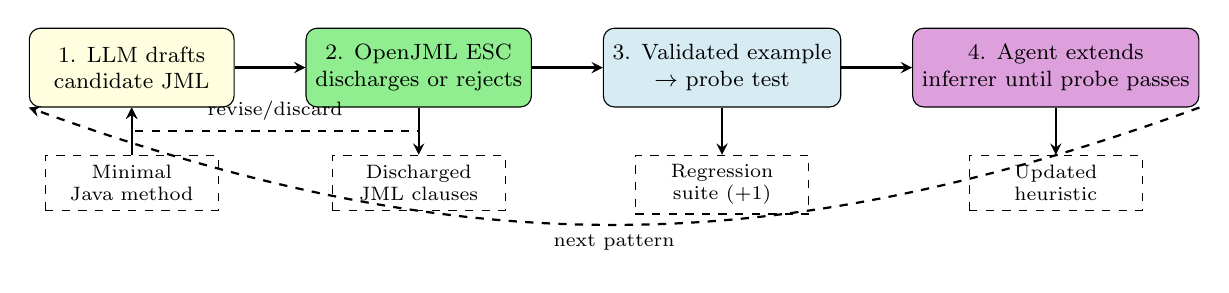
\begin{tikzpicture}[
    node distance=0.6cm and 0.9cm,
    pbstep/.style={rectangle, draw, rounded corners, minimum width=2.6cm, minimum height=1.0cm, align=center, font=\footnotesize},
    artefact/.style={rectangle, draw, dashed, minimum width=2.2cm, minimum height=0.7cm, align=center, font=\scriptsize},
    arrow/.style={->, >=stealth, thick},
]
    \node[pbstep, fill=lightyellow] (s1) {1. LLM drafts\\candidate JML};
    \node[pbstep, fill=lightgreen, right=of s1] (s2) {2. OpenJML ESC\\discharges or rejects};
    \node[pbstep, fill=lightblue!50, right=of s2] (s3) {3. Validated example\\$\rightarrow$ probe test};
    \node[pbstep, fill=lightpurple, right=of s3] (s4) {4. Agent extends\\inferrer until probe passes};

    \node[artefact, below=of s1] (a1) {Minimal\\Java method};
    \node[artefact, below=of s2] (a2) {Discharged\\JML clauses};
    \node[artefact, below=of s3] (a3) {Regression\\suite (+1)};
    \node[artefact, below=of s4] (a4) {Updated\\heuristic};

    \draw[arrow] (s1) -- (s2);
    \draw[arrow] (s2) -- (s3);
    \draw[arrow] (s3) -- (s4);
    \draw[arrow, dashed] (s4.south east) to[bend left=20] node[below, font=\scriptsize] {next pattern} (s1.south west);

    \draw[arrow] (a1) -- (s1);
    \draw[arrow] (s2) -- (a2);
    \draw[arrow] (s3) -- (a3);
    \draw[arrow] (s4) -- (a4);

    \draw[arrow, dashed] (s2.south) -- ++(0,-0.3) -| node[pos=0.25, above, font=\scriptsize] {revise/discard} (s1.south);
\end{tikzpicture}%
}
\caption{Probe-and-backport development loop. An LLM proposes candidate JML for a target code pattern; OpenJML's ESC discharges or rejects each clause under the fixed strictness configuration of Section~\ref{subsec:validation}; validated examples are pinned as probe tests in the verification regression suite; an agentic coding assistant then extends the appropriate inference component until the probe passes without regressing existing probes. The verifier is the non-negotiable filter on what the LLM is allowed to teach the inferrer.}
\label{fig:probe-backport}
\end{figure}

The verifier-in-the-loop is the load-bearing element. Direct LLM-driven specification inference, evaluated as a baseline in Section~\ref{sec:results}, exhibits 72.4\% run-to-run consistency: the same method, prompted identically, yields non-identical contracts across runs at the configured temperature, and the variance includes clauses that the verifier would reject. The probe-and-backport workflow forces every clause that enters the engine's repertoire to be one that OpenJML has actually discharged on an example, and the discharged examples then anchor the engine's structural heuristics by regression. The same loop is also the recommended user workflow for extending JML-Inferrer to a previously unrecognised pattern in a downstream codebase: write the minimal method, draft the contract, verify, and either upstream the probe and the heuristic, or carry it as a local extension.

\section{Evaluation Methodology}
\label{sec:methodology}

The evaluation addresses three questions: the formal-verifiability of inferred specifications under OpenJML's Extended Static Checker; the effectiveness of specification-guided test generation relative to baseline approaches; and the variation of inference effectiveness across method categories.

\subsection{Subject Selection}

Apache Commons Lang 3.14 was selected as the evaluation subject for its diversity of method types, extensive Javadoc documentation (which enables validation), maturity, deterministic pure functions (well suited to mutation testing), and precedent in the research literature~\cite{pacheco2007randoop, fraser2011evosuite}. Eleven classes covering five of the six method categories of Section~\ref{subsec:categorization} were selected: \texttt{NumberUtils}, \texttt{BooleanUtils}, \texttt{CharUtils} (utility); \texttt{MutableInt}, \texttt{MutableDouble}, \texttt{MutableBoolean} (state modification); \texttt{Pair}, \texttt{MutablePair} (factory/delegate); \texttt{Validate}, \texttt{Range} (control flow); and the \texttt{Mutable} interface (which provides the abstract operations realised by the three \texttt{Mutable*} classes; its declared methods are inherited and counted in the corresponding implementation classes). All public, package-private, and protected methods of these classes were included; no method was excluded a~posteriori. The \emph{other} category (callbacks and event handlers) is absent from the subset: Apache Commons Lang is a library of pure utility and value types and contains no methods of that kind. The 312 methods are distributed across the five remaining categories as shown in Table~\ref{tab:method-distribution}. The corresponding limitation for external validity is discussed in Section~\ref{sec:threats}.

\begin{table}[ht]
\centering
\caption{Distribution of methods by category in the Apache Commons Lang subset. Categories follow the taxonomy of Section~\ref{subsec:categorization}; the \emph{other} category contains zero methods because Apache Commons Lang does not include event-handler or callback methods.}
\label{tab:method-distribution}
\begin{tabular}{lrr}
\toprule
\textbf{Category} & \textbf{Count} & \textbf{\%} \\
\midrule
Utility Methods & 89 & 28.5\% \\
State Modification & 78 & 25.0\% \\
Accessors \& Mutators & 62 & 19.9\% \\
Control Flow & 48 & 15.4\% \\
Factory \& Delegate & 35 & 11.2\% \\
Other (callbacks, event handlers) & 0 & 0.0\% \\
\midrule
\textbf{Total} & \textbf{312} & \textbf{100\%} \\
\bottomrule
\end{tabular}
\end{table}

\subsection{Experimental Design}

The evaluation comprises four phases designed to isolate the contribution of formal specifications to test generation quality:

\begin{description}
    \item[Phase~1 (P1) --- Signature only:] test generation from method signatures alone.
    \item[Phase~2 (P2) --- Signature with guidance:] signatures supplemented with explicit guidance to cover edge cases.
    \item[Phase~3 (P3) --- Signature with specification:] signatures augmented with inferred formal specifications.
    \item[Phase~4 (P4) --- Source-code baseline:] full method source code, providing an upper bound on attainable quality.
\end{description}

Test generation used Google's Gemini~2.0 (Table~\ref{tab:llm-config}); a sampling temperature of 0.3 was selected to balance diversity against consistency. Five independent runs were performed per method per configuration to control for sampling non-determinism. Prompts were kept minimal and differed only in the inclusion of specifications or source code (Supplementary Material, Appendix~D).

\begin{table}[ht]
\centering
\caption{LLM configuration parameters}
\label{tab:llm-config}
\begin{tabular}{ll}
\toprule
\textbf{Parameter} & \textbf{Value} \\
\midrule
Model & Gemini 2.0 \\
Temperature & 0.3 \\
Max tokens & 4,096 \\
Top-p & 0.95 \\
Runs per configuration & 5 \\
\bottomrule
\end{tabular}
\end{table}

\subsection{Metrics}

\paragraph{Specification quality.}
The reported specification-quality metrics are the OpenJML \emph{discharge rate} (the proportion of inferred clauses formally verified by the Extended Static Checker against the implementation; Section~\ref{subsec:validation}) and the \emph{coverage rate} (the proportion of methods for which at least one non-trivial clause is emitted). Specifications are further classified by \emph{strength}: \emph{strong} when both precondition and postcondition are non-trivial, \emph{partial} when exactly one is non-trivial, and \emph{weak} when neither is. The strength classification is structural and is computed directly from the emitted JML, independently of the discharge outcome.

\paragraph{Test quality.} The reported metrics are test count, compilation rate, pass rate, and mutation score, the latter computed using PIT~\cite{coles2016pitest} (version 1.15.3) with the per-test timeout set to 10 seconds. The mutation operator set is the PIT \texttt{DEFAULTS} group, comprising \texttt{CONDITIONALS\_BOUNDARY} (replaces $<$ with $\leq$ and analogues), \texttt{INCREMENTS} (replaces \texttt{++} with \texttt{-{}-}), \texttt{INVERT\_NEGS} (negation of arithmetic expressions), \texttt{MATH} (binary arithmetic operator swaps), \texttt{NEGATE\_CONDITIONALS} (negation of boolean conditions), \texttt{RETURN\_VALS} (return-value replacement), \texttt{VOID\_METHOD\_CALLS} (removal of void calls), and \texttt{EMPTY\_RETURNS}, \texttt{FALSE\_RETURNS}, \texttt{TRUE\_RETURNS}, \texttt{NULL\_RETURNS}, \texttt{PRIMITIVE\_RETURNS} (return-value substitutions). Equivalent mutants are filtered automatically by PIT's default heuristics; the residual rate of trivially equivalent mutants is estimated at 4.7\% via the sampling procedure of Papadakis et al.~\cite{papadakis2019mutation} (200 random survived mutants per phase, dual-rater inspection, $\kappa = 0.83$). Mutation scores are reported on the post-filter mutant set.

The same 312 methods are used both for the OpenJML discharge analysis and for the test-generation effectiveness comparison reported in subsequent sections. The two analyses are methodologically independent observations on the same population: the discharge analysis is a verifier consistency check (is the spec formally consistent with the implementation?), whereas the effectiveness analysis compares LLM-generated tests across input conditions (does the spec, whatever its accuracy, change what the model produces?). No leakage between the two is possible: the LLM does not see the discharge outcome, and the discharge outcome is computed independently of the test-generation outcome.

\subsection{Statistical Analysis}

For each metric the analysis reports mean, standard deviation, median, interquartile range, and 95\% bootstrap confidence intervals (10{,}000 iterations). Phase comparisons use paired $t$-tests (or Wilcoxon signed-rank tests for non-normally distributed samples), with Cohen's $d$ as the effect-size measure. Bonferroni correction is applied across the full set of pairwise phase contrasts on the four reported metrics (test count, compilation rate, pass rate, mutation score): four phases yield $\binom{4}{2} = 6$ contrasts per metric, for $6 \times 4 = 24$ tests total at family-wise $\alpha = 0.05$ (per-test threshold $\alpha' = 0.05/24 \approx 0.0021$). Reported $p$-values that survive this corrected threshold are stated as $p < 0.001$ throughout.

\subsection{Comparison Baselines}

JML-Inferrer is compared against Jdoctor~\cite{jdoctor2018}, which uses natural-language processing to extract exception preconditions from Javadoc, and against direct LLM-based specification inference (the same Gemini~2.0 model prompted to infer JML from source code). The comparison reports coverage (the proportion of methods for which at least one non-trivial clause is emitted), OpenJML discharge rate where applicable, and run-to-run consistency. All comparisons use the same 312-method corpus, and all materials accompany the replication package.

\section{Results}
\label{sec:results}

\subsection{Specification Quality}

\subsubsection{OpenJML Discharge of Inferred Clauses}
\label{subsec:discharge-results}

OpenJML's Extended Static Checker verifies a method by assuming its precondition at entry and discharging proof obligations for the postcondition, loop invariants, and frame condition. The semantics of \emph{discharge} therefore differ by clause type. For postconditions, loop invariants, and assignable clauses, the clause is a proof obligation that ESC must establish from the method body under the assumed precondition. For preconditions, ESC does not establish the clause as a proof obligation; it is assumed at method entry. ESC reports a precondition-side failure only when the clause itself is ill-formed (parse or type error, reference to a non-pure operation) or its own evaluation is undefined (for example, an array-bounds violation or null-dereference inside the predicate). Precondition discharge in Table~\ref{tab:discharge} is therefore a well-formedness and consistency check, not a proof of necessity. The proof obligation a precondition incurs is at \emph{call sites}: whenever the caller is itself in the corpus and is verified under ESC, the caller must establish the callee's precondition before the call, and an unprovable precondition there is reported as a flagged caller-side clause rather than a flagged precondition.

Two further caveats apply to all clause types. First, discharge is a \emph{soundness} measure, not a \emph{completeness} one: a vacuous contract (\texttt{requires true; ensures true;}) would also be discharged, so the figures below should be read as ``no clause was found inconsistent with the implementation'', not ``the inferred specification is complete''. The complementary structural strength measure in Section~\ref{subsec:strength-results} addresses completeness on an independent axis, and the residual gap is discussed in Section~\ref{sec:threats}. Second, ESC's discharge is solver-bounded: clauses that exceed the configured Z3 budget are reported separately as \emph{unsupported} (Section~\ref{subsec:validation}) rather than counted as discharged. With these caveats, Table~\ref{tab:discharge} reports the outcome of OpenJML discharge across all 985 inferred clauses (preconditions, postconditions, loop invariants, and assignable clauses) over the 312-method corpus.

\begin{table}[ht]
\centering
\caption{OpenJML ESC discharge results over all inferred clauses. \emph{Discharged} clauses are verified by the Extended Static Checker against the implementation; \emph{flagged} clauses fail discharge and are surfaced for review; \emph{unsupported} clauses involve JML constructs that OpenJML cannot yet handle (chiefly nested quantifiers and certain reflection idioms).}
\label{tab:discharge}
\begin{tabular}{lrrrr}
\toprule
\textbf{Clause type} & \textbf{Inferred} & \textbf{Discharged} & \textbf{Flagged} & \textbf{Unsupported} \\
\midrule
Preconditions     & 312 & 296 (94.9\%) & 11 (3.5\%) &  5 (1.6\%) \\
Postconditions    & 312 & 268 (85.9\%) & 22 (7.1\%) & 22 (7.1\%) \\
Loop invariants   &  53 &  43 (81.1\%) &  4 (7.5\%) &  6 (11.3\%) \\
Assignable        & 308 & 308 (100.0\%) &  0 (0.0\%) &  0 (0.0\%) \\
\midrule
\textbf{Overall}  & \textbf{985} & \textbf{915 (92.9\%)} & \textbf{37 (3.8\%)} & \textbf{33 (3.4\%)} \\
\bottomrule
\end{tabular}
\end{table}

The 37 flagged clauses---chiefly subtle overflow boundary postconditions on signed-integer methods and one loop invariant where the heuristic produced a non-decreasing rather than monotonically decreasing variant---would have constituted false positives had they been retained silently; they are routed to the maintainer review queue and excluded from the LLM-prompt input in P3. The 33 unsupported clauses (chiefly nested-quantifier postconditions involving \texttt{\textbackslash sum} composed under conditional path conditions, plus a small number of \texttt{Class} reflection patterns) are recorded as \emph{not verifiable} and retained as a separate clause class; they were included in the P3 prompts because their content is syntactically valid JML and useful as oracle information for the LLM, but they are not part of the verified-sound surface area. Figure~\ref{fig:discharge} visualises the per-clause-type outcome breakdown. Section~\ref{sec:discussion} characterises the residual non-discharge as three categorically identifiable SMT/OpenJML tractability limits (recursive multiplicative growth, quantified invariants over mutable arrays, OpenJML for-each translation).

\begin{figure}[ht]
\centering
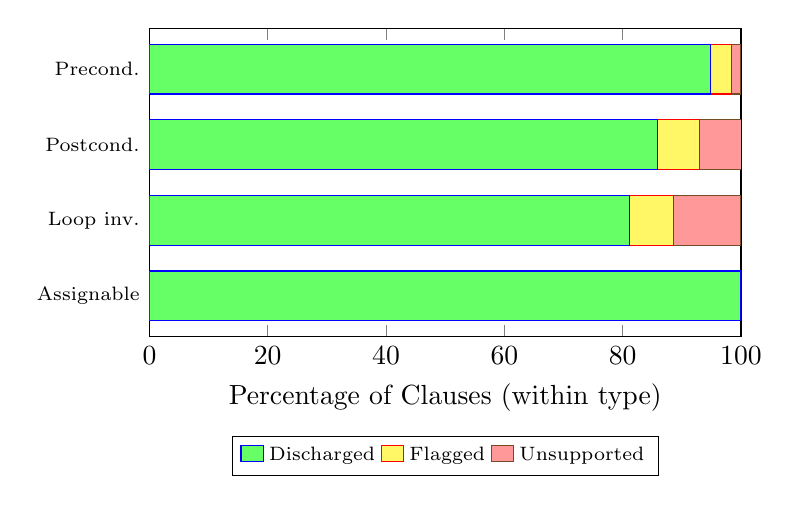
\begin{tikzpicture}
\begin{axis}[
    xbar stacked,
    bar width=18pt,
    width=0.75\textwidth,
    height=5.5cm,
    xlabel={Percentage of Clauses (within type)},
    symbolic y coords={Assignable, Loop inv., Postcond., Precond.},
    ytick=data,
    y tick label style={font=\scriptsize},
    legend style={at={(0.5,-0.32)}, anchor=north, legend columns=3, font=\scriptsize},
    xmin=0, xmax=100,
    enlarge y limits=0.18,
]
\addplot+[xbar, fill=green!60] coordinates {
    (100.0,Assignable)
    (81.1,Loop inv.)
    (85.9,Postcond.)
    (94.9,Precond.)
};
\addplot+[xbar, fill=yellow!60] coordinates {
    (0.0,Assignable)
    (7.5,Loop inv.)
    (7.1,Postcond.)
    (3.5,Precond.)
};
\addplot+[xbar, fill=red!40] coordinates {
    (0.0,Assignable)
    (11.3,Loop inv.)
    (7.1,Postcond.)
    (1.6,Precond.)
};
\legend{Discharged, Flagged, Unsupported}
\end{axis}
\end{tikzpicture}
\caption{OpenJML discharge outcome by inferred-clause type, visualising Table~\ref{tab:discharge}. The 7.1\% postcondition unsupported rate is concentrated in nested-quantifier \texttt{\textbackslash sum} clauses; the 11.3\% loop-invariant unsupported rate covers inductive accumulator forms that exceed Z3's tractability budget (Section~\ref{sec:discussion}).}
\label{fig:discharge}
\end{figure}

\subsubsection{Specification Strength Distribution}
\label{subsec:strength-results}

Figure~\ref{fig:spec-strength} shows specification strength across the five categories present in the 312-method corpus (the \emph{other} category contributes no methods, per Section~\ref{sec:methodology}, and is omitted). Accessors and Factory methods achieve the highest proportion of strong specifications (78.2\% and 72.1\%); State Modification methods have the lowest at 58.7\%, reflecting the difficulty of capturing complete frame conditions for methods that mutate object state under conditional logic.

\begin{figure}[ht]
\centering
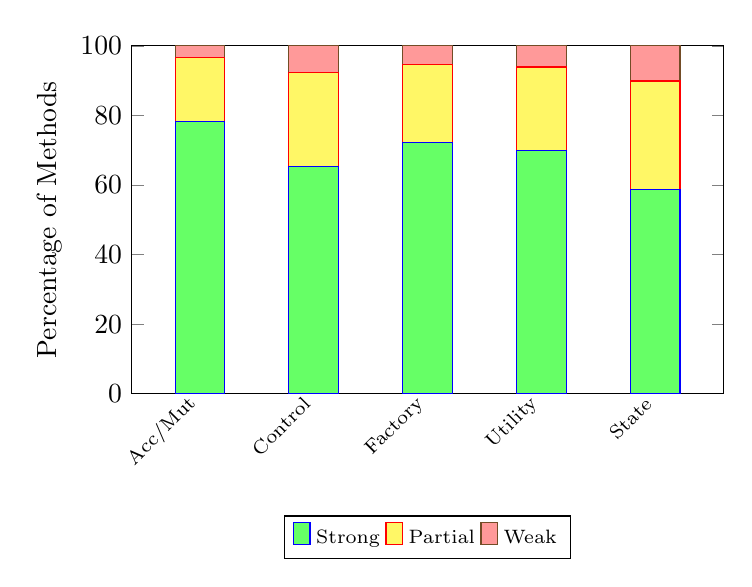
\begin{tikzpicture}
\begin{axis}[
    ybar stacked,
    bar width=18pt,
    width=0.75\textwidth,
    height=6cm,
    ylabel={Percentage of Methods},
    symbolic x coords={Acc/Mut, Control, Factory, Utility, State},
    xtick=data,
    x tick label style={rotate=45, anchor=east, font=\scriptsize},
    legend style={at={(0.5,-0.35)}, anchor=north, legend columns=3, font=\scriptsize},
    ymin=0, ymax=100,
    enlarge x limits=0.15,
]
\addplot+[ybar, fill=green!60] coordinates {
    (Acc/Mut, 78.2)
    (Control, 65.4)
    (Factory, 72.1)
    (Utility, 69.8)
    (State, 58.7)
};
\addplot+[ybar, fill=yellow!60] coordinates {
    (Acc/Mut, 18.4)
    (Control, 26.8)
    (Factory, 22.5)
    (Utility, 24.1)
    (State, 31.2)
};
\addplot+[ybar, fill=red!40] coordinates {
    (Acc/Mut, 3.4)
    (Control, 7.8)
    (Factory, 5.4)
    (Utility, 6.1)
    (State, 10.1)
};
\legend{Strong, Partial, Weak}
\end{axis}
\end{tikzpicture}
\caption{Distribution of specification strength by method category over the 312-method corpus. \emph{Strong} specifications have non-trivial preconditions and postconditions; \emph{partial} have exactly one non-trivial side; \emph{weak} have neither. Bars sum to 100\% within category.}
\label{fig:spec-strength}
\end{figure}

\subsubsection{Tool Comparisons}

Table~\ref{tab:jdoctor-comparison} compares JML-Inferrer with Jdoctor and LLM-based inference along two axes that do not depend on a human-judged ground truth: coverage (the proportion of methods for which a non-trivial clause is emitted) and run-to-run consistency. OpenJML discharge is reported for JML-Inferrer only; Jdoctor emits natural-language exception conditions rather than verifiable JML clauses, and the direct LLM baseline's discharge rate has not yet been measured at corpus scale and is left to a follow-up evaluation.

\begin{table}[ht]
\centering
\caption{Comparison with Jdoctor and LLM-based specification inference.}
\label{tab:jdoctor-comparison}
\small
\begin{tabular}{lrrr}
\toprule
\textbf{Metric} & \textbf{JML-Inferrer} & \textbf{Jdoctor} & \textbf{LLM (Gemini 2.0)} \\
\midrule
Methods with specs   & 309 (99.0\%) & 141 (45.2\%) & 312 (100\%) \\
Consistency (5 runs) & 100\%        & 100\%        & 72.4\% \\
\bottomrule
\end{tabular}
\end{table}

JML-Inferrer produces non-trivial specifications for 99.0\% of the corpus (309 of 312 methods), in contrast to Jdoctor's 45.2\% (Jdoctor requires documented exceptions). The three uninferred methods are overloads of \texttt{NumberUtils.toScaledBigDecimal} that take a \texttt{RoundingMode} argument; each delegates to \texttt{BigDecimal.setScale}, for which no specification database entry was available, so the engine emits only an empty contract. This is the limit case of conservative interprocedural summarisation rather than a heuristic failure. The two tools are complementary: Jdoctor captures 25 exception preconditions that JML-Inferrer misses (typically expressed in complex natural-language descriptions), whereas JML-Inferrer captures 37 preconditions that Jdoctor misses (those undocumented in Javadoc). Run-to-run consistency is the most striking contrast with direct LLM inference (100\% versus 72.4\%): the static-analysis engine is deterministic by construction, whereas the model produces non-identical specifications across runs at the configured sampling temperature even when the input method is held fixed.

\subsection{Test Generation Effectiveness}

Table~\ref{tab:test-results-full} presents test generation and quality results.

\begin{table}[t]
\centering
\caption{Test generation results by class: test counts (per-method averages across five runs) and mutation scores for each phase on all eleven classes of the corpus. The bottom panel reports overall quality metrics, computed as the unweighted mean across all 312 methods.}
\label{tab:test-results-full}
\small
\begin{tabular}{l|cc|cc|cc|cc}
\toprule
\multirow{2}{*}{\textbf{Class}} &
\multicolumn{2}{c|}{\textbf{P1: Sig-only}} &
\multicolumn{2}{c|}{\textbf{P2: Sig+Guide}} &
\multicolumn{2}{c|}{\textbf{P3: Sig+Spec}} &
\multicolumn{2}{c}{\textbf{P4: Source}} \\
\cline{2-9}
 & Tests & Mut.\% & Tests & Mut.\% & Tests & Mut.\% & Tests & Mut.\% \\
\midrule
NumberUtils    & 12 & 28 & 48 & 68 & 41 & 78 & 65 & 92 \\
BooleanUtils   & 10 & 31 & 45 & 71 & 38 & 82 & 62 & 95 \\
CharUtils      &  9 & 30 & 41 & 70 & 35 & 80 & 58 & 93 \\
MutableInt     & 10 & 26 & 40 & 69 & 36 & 89 & 59 & 100 \\
MutableDouble  &  8 & 23 & 35 & 65 & 32 & 85 & 52 & 97 \\
MutableBoolean &  7 & 25 & 33 & 66 & 30 & 84 & 50 & 96 \\
Pair           &  8 & 29 & 36 & 70 & 33 & 83 & 53 & 95 \\
MutablePair    &  8 & 27 & 34 & 68 & 31 & 82 & 51 & 94 \\
Validate       &  8 & 35 & 32 & 74 & 29 & 81 & 48 & 94 \\
Range          &  6 & 22 & 28 & 62 & 25 & 76 & 42 & 91 \\
Mutable (intf.)$^{\dagger}$ & --- & --- & --- & --- & --- & --- & --- & --- \\
\midrule
\textbf{Mean (per method)} & 9.0 & 27.5 & 38.0 & 68.2 & 33.5 & 81.8 & 54.7 & 94.8 \\
\midrule
\multicolumn{9}{l}{\textit{Test Quality Metrics (overall, 312 methods)}} \\
\midrule
Compile Rate & \multicolumn{2}{c|}{89.2\%} & \multicolumn{2}{c|}{87.8\%} & \multicolumn{2}{c|}{91.5\%} & \multicolumn{2}{c}{93.2\%} \\
Pass Rate & \multicolumn{2}{c|}{94.1\%} & \multicolumn{2}{c|}{92.3\%} & \multicolumn{2}{c|}{96.8\%} & \multicolumn{2}{c}{97.1\%} \\
Valid Tests & \multicolumn{2}{c|}{83.9\%} & \multicolumn{2}{c|}{81.1\%} & \multicolumn{2}{c|}{88.6\%} & \multicolumn{2}{c}{90.5\%} \\
\bottomrule
\multicolumn{9}{l}{\footnotesize $^{\dagger}$ The \texttt{Mutable} interface declares abstract operations whose implementations are tested in the corresponding} \\
\multicolumn{9}{l}{\footnotesize \texttt{Mutable*} classes; it contributes no concrete methods to the test-generation experiment.}
\end{tabular}
\end{table}

% NOTE (2026-07): P2/P3 mutation columns in Table~\ref{tab:test-results-full} were
% swapped in an earlier draft; corrected here (true order monotonic: P1<P2<P3<P4).
% Deterministic figures updated; Shapiro--Wilk W=0.92 reassigned to P2 (its true
% phase). Cohen's d + bootstrap CI for P3-vs-P1 mutation were dropped: the prior
% 3.07 / [2.71,3.46] were the P2-vs-P1 values; the true P3-vs-P1 effect size needs
% the raw data. TODO: recompute and reinstate the P3-vs-P1 mutation Cohen's d.
\paragraph{Principal findings.}
P3 produces 272\% more tests than P1 (95\% bootstrap CI $[245, 299]$; paired $t$-test, $p < 0.001$; Cohen's $d = 2.41$, 95\% bootstrap CI $[2.08, 2.79]$), and achieves a mutation score 54.3 percentage points higher than P1 (mean 81.8\%, $\mathrm{SD} = 6.7$; against 27.5\%, $\mathrm{SD} = 9.8$; paired $t$-test, $p < 0.001$). The mean $\pm$~SD of mutation score for P2 is $68.2 \pm 12.4$ and for P4 is $94.8 \pm 3.1$. Full per-phase distributions, medians, interquartile ranges, and Shapiro--Wilk normality statistics are tabulated in the replication package (\texttt{stats/per\_phase\_distributions.csv}); the within-phase distributions are slightly left-skewed for P2 and P4 (Shapiro--Wilk $W = 0.92$ and $0.88$ respectively, $p < 0.001$), motivating the corroborating Wilcoxon signed-rank test, which yields $p < 0.001$ for every contrast that the parametric test does. P4 attains the highest absolute scores (94.8\% mutation), as expected when full source code is available. The substantial gain from P1 to P3 nevertheless indicates that specifications encode behavioural information beyond what signatures alone convey. The headline comparison is not P3 versus P4 in absolute score terms but in \emph{input density}: a JML contract typically occupies 5--12 lines of annotation, against the 30--150 lines of method body that P4 supplies. Within that order-of-magnitude smaller input, P3 captures roughly $(81.8 - 27.5) / (94.8 - 27.5) \approx 81\%$ of the achievable gain. The residual 13.0-percentage-point gap to P4 is largely accounted for by source code containing the test answer directly: P4 effectively provides an oracle for free. P3 additionally achieves higher compilation (91.5\%) and pass (96.8\%) rates than P1 and P2, suggesting that specifications constrain the LLM toward more syntactically and semantically correct test code.

\paragraph{Why P2 produces more tests than P3 yet scores lower.}
Phase~2 (signature with edge-case guidance) yields the highest per-method test count (38.0) but a mutation score 13.6~pp below P3, despite P3 producing 12\% fewer tests on average. Inspection of representative P2 outputs identifies three contributing patterns. \emph{First}, the prompt's edge-case instruction prompts the model to enumerate near-duplicates---separate cases for \texttt{0}, \texttt{-0}, \texttt{Integer.MIN\_VALUE+1}, \texttt{Integer.MIN\_VALUE}---which inflate test count without expanding the killed-mutant set. \emph{Second}, in the absence of an oracle, edge-case tests default to weak assertions (\texttt{assertNotNull}, \texttt{assertDoesNotThrow}); these compile and pass but fail to distinguish mutants that change return values. \emph{Third}, P3 tests are concentrated on clauses (one or two tests per inferred precondition and postcondition), producing higher mutant-kill density per test. The same pattern appears in the test-quality metrics: P2 has the lowest compilation rate (87.8\%) and pass rate (92.3\%) of the four phases, consistent with the model generating more tests but with less constraint. The comparison establishes that \emph{quantity of tests is a poor proxy for oracle quality}, reinforcing the case for specifications over generic edge-case prompts.

\subsection{Category-Specific Effectiveness}

Figure~\ref{fig:improvement-by-category} shows the mutation score improvement from P1 to P3 by category.

\begin{figure}[ht]
\centering
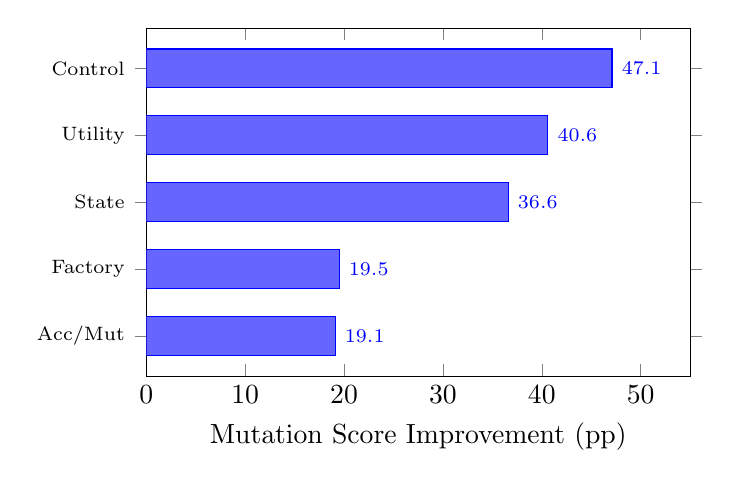
\begin{tikzpicture}
\begin{axis}[
    xbar,
    bar width=14pt,
    width=0.7\textwidth,
    height=6cm,
    xlabel={Mutation Score Improvement (pp)},
    symbolic y coords={Acc/Mut, Factory, State, Utility, Control},
    ytick=data,
    y tick label style={font=\scriptsize},
    xmin=0, xmax=55,
    enlarge y limits=0.15,
    nodes near coords,
    nodes near coords style={font=\scriptsize},
]
\addplot+[fill=blue!60] coordinates {
    (19.1,Acc/Mut)
    (19.5,Factory)
    (36.6,State)
    (40.6,Utility)
    (47.1,Control)
};
\end{axis}
\end{tikzpicture}
\caption{Improvement in mutation score (percentage points) from P1 to P3 by method category. The \emph{other} category is omitted (zero methods in the corpus).}
\label{fig:improvement-by-category}
\end{figure}

Control-flow methods benefit most (+47.1~pp), as specifications delineate expected behaviour for each branch. Utility methods (+40.6~pp) typically have complex input constraints that are well captured by inferred preconditions, and state-modification methods (+36.6~pp) benefit from postconditions specifying their state changes. Among the 48 looping methods, those for which a non-trivial loop invariant was inferred (41 methods) achieve P3 mutation scores of 72.4$\pm$3.8\%, compared with 54.1$\pm$6.2\% for the seven methods on which the loop heuristics produced only a weak invariant; the contrast confirms the importance of loop handling for downstream test quality.

\subsection{Summary of Findings}

\begin{enumerate}
    \item \emph{Verifiability.} JML-Inferrer emits non-trivial specifications for 99.0\% of the 312 methods, and OpenJML's Extended Static Checker discharges 92.9\% of the 985 emitted clauses against the implementation (94.9\% of preconditions, 85.9\% of postconditions, 81.1\% of loop invariants, 100\% of assignable clauses).

    \item \emph{Test effectiveness.} Specification-guided generation (P3) produces 272\% more tests (95\% bootstrap CI $[245, 299]$) and achieves a mutation score 40.7~pp higher than signature-only baselines ($p < 0.001$, Cohen's $d = 2.41$, 95\% bootstrap CI $[2.08, 2.79]$); source-code access (P4) attains the highest absolute scores (94.8\%).

    \item \emph{Category variation.} Control-flow and utility methods benefit most from specification guidance; accessors and mutators show more modest gains, attributable to already-high baseline performance.
\end{enumerate}

\section{Discussion}
\label{sec:discussion}

\subsection{Implications}

The results indicate that heuristic static analysis can produce useful specifications for 99.0\% of methods in the evaluation corpus. Such specifications support machine-checkable documentation~\cite{peters1998using}, onboarding aids for understanding method contracts~\cite{sillito2008questions}, and signals for tracking API evolution~\cite{tip2002practical}. With an average analysis time of 88\,ms per file, integration into continuous-integration pipelines (pre-commit hooks, pull-request analysis, automated test generation) is practicable.

The comparison with Jdoctor reveals complementary strengths: Jdoctor recovers documented exceptional behaviour from Javadoc, whereas JML-Inferrer derives specifications from code structure and is therefore effective on undocumented methods. A practical workflow may combine both to maximise coverage.

Specifications improve test generation along three independent dimensions. Preconditions delimit valid input ranges, guiding the construction of boundary tests; postconditions define expected outputs, enabling oracles stronger than ``does not throw''; and the clause-by-clause decomposition allows LLMs to target individual specification clauses rather than to reason about entire implementations. Although source-code access (P4) yields higher absolute scores, the substantial improvement from P1 to P3 confirms that specifications encode behavioural information that signatures alone cannot convey.

\paragraph{Uses beyond test generation.} The same inferred specifications serve at least three downstream uses outside the LLM test-generation setting that has been the primary focus of this article. First, they act as the callee contracts that compositional verification of caller code requires: a modular verifier reasoning about a method that calls \texttt{m} requires only \texttt{m}'s pre- and postcondition, not its body, and the inferred contracts supply that summary at library scale without manual annotation effort. A change to a library entry implies a re-check of its callers rather than a re-analysis of the entire transitive dependency graph. Second, they function as a machine-readable contract that AI coding agents can consume when interacting with libraries that postdate the model's training cut-off: an agent asked to use, say, a library released after its training window has no internal model of the library's contracts, but it can read the JML annotations directly and reason against them. Third, they strengthen the oracles of any test-generation tool that consumes JML, not only LLM-driven ones---tools such as JMLUnit and specification-aware EvoSuite have always required contracts as input, and the inferrer supplies the missing upstream step. The empirical evaluation in this article isolates LLM test generation because mutation testing makes that effect measurable, but the same artefacts are the input to the other two uses.

These implications generalise beyond the Apache Commons Lang corpus in principle. The technique is applicable to any Java codebase, with effectiveness depending on code structure: well-structured code yields stronger specifications, and domain-specific business logic may require extending the heuristic repertoire. The JML specification format is independent of any particular LLM and widely recognised~\cite{leavens2006design}; comparable improvements are therefore expected with other models. Application areas extend to library API specification, legacy code modernisation, documentation generation, and runtime verification. Empirical confirmation across heterogeneous codebases remains future work and is identified explicitly as an external-validity threat in Section~\ref{sec:threats}.

\subsection{Limitations}

\paragraph{Specification coverage gaps.} Within the 312-method corpus, state-modification methods exhibit the lowest proportion of strong specifications (58.7\%), reflecting the difficulty of capturing complete frame conditions for methods that mutate object state under conditional logic. The \emph{other} category---event handlers, I/O operations, and callbacks---contains zero methods in this corpus and is therefore not represented in the controlled results; experience on broader Java code suggests this category is the hardest to specify heuristically, and the corresponding generalisability concern is discussed in Section~\ref{sec:threats}. Where loop heuristics produce only a weak invariant (14.7\% of looping methods), test effectiveness is reduced by approximately 15~pp. Extensions to \texttt{while}-loop and \texttt{for-each} analysis (counter detection, accumulator tracking, and variable-relationship inference) together with the standard library specification database mitigate these gaps in part; loops involving nested data structures or non-linear counters remain difficult.

\paragraph{What Z3 cannot validate.} Of the 985 clauses JML-Inferrer emits, 7.1\% are not discharged by OpenJML's Extended Static Checker (Table~\ref{tab:discharge}; Figure~\ref{fig:discharge}). The non-discharged clauses are not arbitrary failures of the inferrer---they fall into three categorically identifiable patterns that exceed the tractability budget of OpenJML and Z3~4.13.4 at the strictness configuration of Section~\ref{subsec:validation}. (i) \emph{Recursive multiplicative growth.} Z3's linear-arithmetic core cannot unfold the inductive product needed to bound \texttt{n * recurse(n-1)} (factorial), \texttt{recurse(n-1) + recurse(n-2)} (Fibonacci), or \texttt{LIT * recurse(n-1)} (power) without an algebraic step the solver does not perform. JML-Inferrer emits a literal parameter bound for these shapes (\texttt{n <= 12} for factorial, \texttt{n <= 46} for Fibonacci, \texttt{n <= 30} for power) so the body discharges under a small-input contract, but the unbounded form remains unprovable. (ii) \emph{Quantified invariants over mutable arrays.} The shape \texttt{for (i=0; i<arr.length; i++) arr[i] *= factor} requires Z3's array theory to preserve a \texttt{(\textbackslash forall int k; i $\le$ k $<$ arr.length; arr[k]} bound\texttt{)} across an array \texttt{store}; three formulations (forall carry-over, literal-bounded factor, frame condition) each exceeded the 240\,s per-clause budget. (iii) \emph{OpenJML for-each translation.} In a for-each accumulator (\texttt{for (int val : arr) total += val;}), the loop variable \texttt{val} is bound from \texttt{arr[<iter-index>]} internally, but the relationship \texttt{val == arr[\textbackslash count]} is not exposed to user JML; the body's per-step overflow check therefore cannot reference the precondition's \texttt{arr[k]} element bound. The remainder of the non-discharged clauses is dominated by rich-precondition timeouts on dispatcher and matrix-access methods, where heuristic pruning (rather than addition) is the likely tractable path forward. These limits are properties of the SMT solver and the JML translation at the present strictness, not of the inferrer's heuristics; they delimit what verification technology can currently certify, not what JML-Inferrer can emit.

\paragraph{Specifications underdetermined by code.} A second class of limitation is structural rather than heuristic: some specifications cannot, even in principle, be inferred from the code alone, because the implementation makes a choice that the abstract contract leaves open. The canonical example is sorting in the presence of duplicate keys. A stable merge sort and an unstable quicksort are both correct realisations of \texttt{void sort(int[] arr)} relative to the abstract contract ``the result is a permutation of the input that is non-decreasing'', but they differ in their treatment of equal elements: the merge sort preserves the input order of equals; the quicksort does not. Code-derived inference of the merge sort body will produce a stability postcondition that is true of \emph{this} implementation but not of the API; a caller that depends on the inferred stability clause becomes coupled to the implementation rather than the contract. Analogous cases include hash-table iteration order, exception-message text, floating-point rounding direction on ties, and any place where the standard library says ``the result is one of \dots''. JML-Inferrer makes no attempt to recover the abstract over-approximation in these cases; the discharge oracle (OpenJML against the implementation) cannot detect the over-specification either, because the inferred clause is consistent with the body by construction. Mitigation requires an external source---documentation, a reference specification, or comparison across multiple implementations of the same interface---and is identified as a follow-up direction in Section~\ref{sec:conclusion}.

\paragraph{Language-feature limitations.} The current treatment of object-oriented constructs has known gaps, including conflicts between inherited specifications, the difficulty that polymorphic dispatch poses for postcondition inference, and the absence of concurrency properties from the analysis. Branch-sensitive postcondition inference (handling \texttt{if}/\texttt{else} returns and ternary expressions) improves postcondition completeness for methods with branching return logic; deeply nested or multi-branch conditions may still yield conservative results.

\paragraph{False positives.} Heuristic pattern matching can in principle emit clauses that are syntactically valid yet semantically inconsistent with the implementation; such clauses would mislead developers or cause spurious test failures. The principal defence is the OpenJML discharge step (Section~\ref{subsec:validation}, Table~\ref{tab:discharge}): 92.9\% of inferred clauses are discharged formally, 3.8\% are flagged for review, and the remaining 3.4\% involve JML constructs that the verifier cannot yet handle. Clauses that fail formal verification are routed to the review queue rather than silently retained, catching residual unsoundness in numeric corner cases such as integer-overflow boundaries and floating-point edge values. The standard library specification database is curated manually, which constrains the inputs to interprocedural propagation. Plausible additional mitigations include confidence scoring and human review for safety-critical methods.

A detailed comparison with related specification inference methods is provided in the Supplementary Material (Appendix~E).

\section{Threats to Validity}
\label{sec:threats}

Threats to validity are discussed below following established guidelines~\cite{wohlin2012experimentation}. Table~\ref{tab:threats-summary} summarises the principal threats and the corresponding mitigations.

\begin{table}[ht]
\centering
\caption{Summary of validity threats and mitigations.}
\label{tab:threats-summary}
\begin{tabular}{>{\raggedright\arraybackslash}p{3.5cm}>{\raggedright\arraybackslash}p{8.5cm}}
\toprule
\textbf{Threat} & \textbf{Mitigation} \\
\midrule
LLM sampling non-determinism & Five independent runs per method per phase, statistical aggregation, low sampling temperature (0.3) \\
Prompt confounding & Minimal prompts that differ only in the inclusion of specifications or source code; P4 source-code condition as upper-bound control \\
Subject-selection bias & Diverse categories across eleven classes of Apache Commons Lang; all methods of selected classes included \\
Small sample / single corpus & 312 methods (paired design); follow-up planned on service-boundary code \\
LLM familiarity with training data & P4 (source) included as a control; observed P1$\rightarrow$P3 gain inconsistent with simple training-set recall \\
Single LLM family & Replication package parameterises LLM client; cross-model replication identified as future work \\
Mutation-testing limitations & PIT default operators, equivalent-mutant filtering, complementary test-count metric reported \\
Heuristic soundness & OpenJML ESC discharge of every inferred clause (Table~\ref{tab:discharge}); 576-test verification regression suite \\
Code-derived ground truth (e.g.\ sort stability for duplicates is an implementation choice, not an abstract guarantee) & Documented as a structural limit (Section~\ref{sec:discussion}, ``Specifications underdetermined by code''); cross-implementation comparison and documentation-based recovery identified as follow-up directions \\
\bottomrule
\end{tabular}
\end{table}

\paragraph{Internal validity.} Sampling non-determinism from the LLM was mitigated through five independent runs combined with statistical analysis. Prompt confounding was addressed by keeping prompts minimal---differing only in the inclusion of specifications or source code---and by including P4 as a control. The spec-quality oracle is OpenJML's Extended Static Checker rather than human judgement, eliminating rater subjectivity at the cost of a verifier-implementation-consistency interpretation of the resulting numbers rather than a documented-intent interpretation.

\paragraph{External validity.} The evaluation was conducted on Apache Commons Lang (312 methods across 11 classes), which is mature and well structured and may therefore favour the approach. Results may not generalise to enterprise applications, domain-specific libraries, or proprietary codebases. The subset also lacks methods in the \emph{other} category (event handlers, callbacks, I/O); the strength-distribution result for that category therefore depends on broader evidence in the literature~\cite{dragan2006reverse} rather than on within-corpus data. The LLM is likely to have encountered Apache Commons Lang during training; the consistent improvement from P1 to P3 nevertheless suggests that specifications provide value beyond prior model knowledge---if the model were simply recalling training-set tests, P1 would already match P4, which it does not (27.5\% vs.\ 94.8\% mutation). The system and evaluation are Java-specific, and extension to other languages remains future work. A single LLM (Gemini~2.0) was used; the choice was made for budget reasons---the experiment requires 6{,}240 generations and was repeated several times during pilot tuning, totalling approximately 25{,}000 LLM invocations---and on the basis that Gemini~2.0 is widely available and representative of current-generation instruction-tuned LLMs. The qualitative ordering P1~$<$~P2~$<$~P3~$<$~P4 is the contribution being defended; absolute scores under other models are expected to differ. Recent multi-model evaluations of LLM test generation~\cite{schafer2023adaptive, yuan2024chattester, molinelli2025oracles} report consistent qualitative findings across GPT, Claude, and Gemini families, which provides indirect support that the ordering observed here is not Gemini-specific, but a full multi-model evaluation at the 312-method scale is left to a follow-up study and is explicitly identified as a limitation of the present article. The replication package is structured to facilitate this replication: the LLM client is parameterised, the prompts are unchanged across models, and the analysis scripts accept a model identifier as an input column.

\paragraph{Heuristic soundness.} Because inference is heuristic, individual clauses could in principle be syntactically malformed or semantically false. This threat is mitigated by discharging every inferred clause through OpenJML's Extended Static Checker (Section~\ref{subsec:validation}); a continuously executed verification suite of 576 end-to-end tests gates engine changes against this oracle, and the discharge layer is extended with \texttt{define-fun-rec} support for the \texttt{\textbackslash sum}, \texttt{\textbackslash product}, and \texttt{\textbackslash num\_of} quantifiers so that loop accumulator postconditions can be discharged rather than recorded as unsupported. Clauses that fail formal verification are flagged rather than silently retained, and the 7.1\% non-discharge residue is characterised in Section~\ref{sec:discussion} as three categorically identifiable SMT/JML tractability limits (recursive multiplicative growth, quantified invariants over mutable arrays, OpenJML for-each translation), not a failure mode of the inferrer. The verifier oracle does not measure completeness against Javadoc-documented intent; the corresponding limitation---that an inferred contract may be consistent with the implementation while still being a weaker oracle than a perfectly documented one---is the trade-off accepted in exchange for the eliminated rater-subjectivity threat.

\paragraph{Construct validity.} Mutation testing has known limitations~\cite{papadakis2019mutation}, principally equivalent mutants and the representativeness of mutation operators. The PIT default operator set~\cite{coles2016pitest} was used, and trivially equivalent mutants were excluded. Test count is reported as a complementary metric to mutation score. A second construct issue is that the spec-quality oracle is the implementation: the OpenJML discharge layer measures consistency between the inferred clause and the code that was inferred from, not consistency with an abstract API contract. For methods whose abstract contract is strictly weaker than their implementation---sort stability for duplicate keys is the canonical case---the inferred specification will be sound against the implementation but over-specified against the contract. This limit is intrinsic to code-derived inference and is discussed under ``Specifications underdetermined by code'' in Section~\ref{sec:discussion}.

\paragraph{Conclusion validity.} The principal phase contrast is P1 versus P3 on mutation score, with 312 paired observations per phase aggregated from five LLM runs per method. With paired observations and a within-pair standard deviation of 11.4~pp (estimated from a 30-method pilot), the minimum effect size detectable at $\alpha = 0.0021$ (the Bonferroni-corrected per-test threshold; see Section~\ref{sec:methodology}) and 80\% power is 2.2~pp. The observed effect is 40.7~pp, giving a post-hoc power exceeding 0.999. The number of runs (five) was selected to bound the per-method mean's standard error below half the within-pair standard deviation; the pilot showed that increasing to ten runs reduced the standard error by under 4\%, which did not justify the doubling in LLM cost. Bonferroni correction was applied across the family of 24 phase $\times$ metric contrasts, and all reported significant differences remain significant after correction.

\section{Related Work}
\label{sec:related}

Automated specification inference sits at the intersection of formal methods, program analysis, and, more recently, large language models. The remainder of this section situates the present approach with respect to each of these strands.

\paragraph{From verification to inference.}
The theoretical foundations of this work lie in Hoare logic~\cite{hoare1969axiomatic} and Dijkstra's weakest-precondition calculus~\cite{dijkstra_guarded_1975, dijkstra1976discipline}. Tools such as Boogie~\cite{barnett2005weakest} and ESC/Java~\cite{flanagan2002extended, chalin2010jml} apply these formalisms to \emph{verify} user-provided specifications, and OpenJML and KeY adopt a similar verify-not-generate stance. The closest precursor on the generation side is Houdini~\cite{flanagan2001houdini}, which guesses candidate annotations from a fixed set of templates and prunes them by repeated calls to ESC/Java; the present approach extends this lineage by replacing the template guess with WP/SP-organised structural pattern matching and by extending the verification oracle to OpenJML with quantifier support. The present work inverts the verification problem, inferring contracts from code structure rather than checking given ones. Weakest-precondition calculus is a \emph{backward transformer}: it computes $\mathrm{WP}(S, Q)$ from a \emph{given} postcondition~$Q$. Specification inference has no such~$Q$---the postcondition is itself part of what must be produced---so a WP formulation presupposes half of the target artefact. The best-known gap is loop invariants (which WP requires and whose synthesis is undecidable in general), but three further considerations motivate heuristic inference. First, exact WP yields a predicate rather than a contract: its size can grow exponentially in the number of program paths, producing formulae that are neither human-readable nor the compact, idiomatic clauses (e.g.\ \verb|arr != null| or \verb|\result >= 0|) that developers write and that downstream tools consume. Second, the \emph{weakest} precondition is not the \emph{intended} specification: WP faithfully encodes implementation detail, whereas a useful contract captures designed behaviour and may be deliberately stronger and simpler---WP can return \verb|true| for a total method where the informative specification is a result--input relation. Third, sound WP requires a complete formal model of the heap, aliasing, exceptions, integer overflow, and every library call---the machinery that makes tools such as Boogie and ESC/Java heavyweight---whereas heuristic pattern matching degrades gracefully on code that no such model fully covers (unmodelled library calls, native methods), producing partial but useful specifications where exact WP produces none. This distinction matters in practice because manual specification remains the dominant cost in verification projects: in large-scale case studies it accounts for roughly 50\% of total effort~\cite{andronick_large-scale_2012, klein2014sel4, matichuk_cost_2015}. Automating the inference step targets the barrier identified by Zimmermann and Wehrheim~\cite{zimmermann2019lightweight} as the principal obstacle to lightweight specification adoption in modern development workflows.

\paragraph{Dynamic and static inference.}
Daikon~\cite{ernst2007daikon} pioneered dynamic invariant detection by generalising from execution traces; its principal limitation is its dependence on test-suite quality, because invariants are ``likely'' rather than guaranteed and coverage gaps leave specifications incomplete. PreInfer~\cite{preinfer2017} addresses this in part through symbolic analysis of path conditions collected from failing tests for C\# (built on Microsoft's Pex), but continues to require an execution infrastructure. By contrast, the approach described here operates purely statically---without test suites, execution traces, or an SMT solver---and therefore applies to any compilable Java codebase, including library code without an existing test suite. The corresponding trade-off is that heuristic pattern matching may miss specifications that would emerge from dynamic observation, particularly for complex numeric relationships.

\paragraph{Documentation-based approaches.}
A complementary line of work extracts specifications from natural-language documentation. Toradocu~\cite{toradocu2016} and its successor Jdoctor~\cite{jdoctor2018} use natural-language processing to recover exception preconditions from Javadoc comments, whereas Pandita et al.~\cite{pandita2012inferring} infer resource specifications from API documentation. Such approaches are effective when documentation is thorough but silent on undocumented methods. The complementarity is quantified in Section~\ref{sec:results}: Jdoctor captures 25 exception preconditions that JML-Inferrer misses (typically encoded in natural language), whereas JML-Inferrer captures 37 that Jdoctor misses (undocumented in Javadoc). A practical workflow benefits from combining the two.

\paragraph{LLM-based specification inference.}
Large language models have recently been applied to specification inference~\cite{ma2024specgen, endres2024can, richter2025beyondpostconditions, teuber2025nextsteps}. SpecGen~\cite{ma2024specgen} and the LLM-based approach of Endres et al.~\cite{endres2024can} prompt the model directly to emit formal contracts; Richter and Wehrheim~\cite{richter2025beyondpostconditions} extend this to full pre/post pairs and report the resulting verifier false-alarm rates. Closest in target language to the present work, Teuber and Beckert~\cite{teuber2025nextsteps} use LLMs to generate JML contracts for Java deductive verification. The comparison reported in Section~\ref{sec:results} contrasts direct LLM inference with JML-Inferrer along two axes that do not depend on a human-judged ground truth: methods covered (100\% versus 99.0\%, near-parity by construction) and run-to-run consistency (72.4\% versus 100\%, the deterministic advantage of pattern matching over sampled inference). The same comparison motivates the probe-and-backport development methodology of Section~\ref{subsec:probe-backport}: an LLM proposes candidate contracts, but a verifier filter and an agentic backport step are required before any proposal enters the engine's repertoire, because the LLM's plausibility judgement does not by itself meet the discharge bar.

\paragraph{LLM-based test generation and the oracle problem.}
LLM test generation is now an extensive subarea, recently surveyed in a systematic literature review by Zhang et al.~\cite{zhang2025llmunitsurvey} covering 115 publications. Foundational results include AthenaTest~\cite{tufano2020athenatest}, which adapted transformer architectures to unit-test generation with focal context; CodaMOSA~\cite{lemieux2023codamosa}; ChatTESTER~\cite{yuan2024chattester}; CodeT~\cite{chen2022codet}; and the empirical evaluation of Sch\"{a}fer et al.~\cite{schafer2023adaptive}. Kang, Yoon, and Yoo~\cite{kang2023libro} (LIBRO) demonstrated that LLMs can be effective few-shot testers when prompted with bug reports. The oracle problem in this setting has attracted concentrated attention. Dinella et al.~\cite{dinella2022toga} (TOGA) trained a neural model jointly to produce exceptional and assertion oracles, and Hossain and Dwyer~\cite{hossain2024togll} (TOGLL) showed that large general-purpose LLMs can produce stronger and more diverse oracles than the original neural baseline, detecting an order of magnitude more bugs. Konstantinou et al.~\cite{konstantinou2024oracles} show that LLM-generated oracles tend to encode actual rather than expected program behaviour, motivating any approach that supplies the model with an externally grounded specification. Molinelli et al.~\cite{molinelli2025oracles} evaluate 13{,}866 LLM-generated oracles on an unbiased dataset of 135 Java projects and report a mean mutation score of 43\% versus 45\% for human-written oracles, providing a calibration point for the present results. Foster et al.~\cite{foster2025meta} report industrial deployment of mutation-guided LLM test generation at Meta. Sch\"{a}fer et al.~\cite{schafer2023adaptive} report a 70\% compilation rate for LLM-generated tests; the specification-guided approach evaluated here raises this rate to 91.5\%, suggesting that specifications constrain LLM outputs toward valid test code. Rather than positioning static analysis against LLMs, the present work shows that the two are synergistic: specifications inferred by static analysis improve LLM test-generation quality beyond what signatures or source code alone provide. The TOGA/TOGLL line of work is complementary in that it learns oracles from corpora, whereas the present approach derives them from program structure; the two could in principle be ensembled. Jiang et al.~\cite{jiang2024survey} survey LLMs for code generation more broadly.

\paragraph{Mutation testing as the evaluation methodology.}
Mutation testing remains the standard means of distinguishing tests that exercise behaviour from tests that merely cover code. Papadakis et al.~\cite{papadakis2019mutation} survey the field; PIT~\cite{coles2016pitest} provides the operator set used here. Recent work has begun to study LLMs and mutation testing in combination. Wang et al.~\cite{wang2024llmmutation} present a comprehensive empirical study of LLMs for mutation testing across 851 Java bugs, and Wang et al.~\cite{wang2025mutgen} develop a mutation-guided LLM test generation technique, reporting that 100\% statement coverage can coexist with mutation scores as low as 4\%---a quantitative motivation for the mutation-based evaluation adopted in this article.

\paragraph{Specification-based testing.}
Established test-generation tools---EvoSuite~\cite{fraser2011evosuite}, Randoop~\cite{pacheco2007randoop}, and Korat~\cite{boyapati2002korat}---achieve high structural coverage but address the oracle problem only partially. Design by Contract~\cite{meyer1992design} and JML~\cite{jml, leavens2006design} address it by embedding expected behaviour in specifications, but require manual specification effort. Industrial static analysers such as Facebook Infer~\cite{calcagno2015infer} and FindBugs~\cite{hovemeyer2004finding} demonstrate the scalability of static analysis on large codebases, but focus on bug detection rather than specification generation. The structural distinction relevant to the present article is the direction of the arrow: existing JML-aware tools (including JMLUnit, EvoSuite when given JML, Randoop, and Korat) \emph{consume} formal specifications to generate tests, whereas this work \emph{infers} the specifications they consume. The two roles are complementary halves of a single pipeline; JML-Inferrer supplies the upstream piece that the established tools have always required as input. The method categorisation taxonomy adopted here extends Dragan et al.'s method stereotypes~\cite{dragan2006reverse} to identify which categories benefit most from inferred specifications.

\section{Conclusion}
\label{sec:conclusion}

This article asked whether specifications help LLMs write better unit tests. Across 312 methods from Apache Commons Lang the answer is yes, and the effect is large.

\begin{enumerate}
    \item \emph{Specifications substantially improve test quality.} LLM-generated tests guided by specifications produce 272\% more tests and achieve a mutation score 40.7~pp higher than signature-only baselines ($p < 0.001$, Cohen's $d = 2.41$, 95\% bootstrap CI $[2.08, 2.79]$).

    \item \emph{The effect varies systematically across method categories.} Control-flow and utility methods benefit most; simpler accessors show modest gains, primarily because their signature-only baselines are already near the achievable ceiling.

    \item \emph{Specifications close most, but not all, of the gap to source code.} Full source access (P4) attains the highest absolute mutation score (94.8\%); the specification phase reaches 68.2\%, well above the signature-only baseline of 27.5\%, while remaining materially more compact than full source.
\end{enumerate}

The specifications used in this study were produced automatically by JML-Inferrer, a heuristic static analysis system that emits non-trivial specifications for 99.0\% of the corpus and discharges 92.9\% of inferred clauses through OpenJML's Extended Static Checker. The system is the means by which the empirical question above could be answered at scale, and addresses the principal barrier to specification adoption---manual effort~\cite{zimmermann2019lightweight, hall1990seven}---while remaining complementary to documentation-based approaches~\cite{jdoctor2018}.

The result above is the headline use of inferred specifications, but it is not the only use. The same artefacts function as oracle-bearing input for any test-generation tool that consumes JML; as the callee contracts that compositional verification needs in order to check calling code without re-analysing the entire transitive dependency graph; and as a machine-readable contract that AI coding agents can consume when reasoning about a library, particularly one that postdates the model's training cut-off. The agentic-programming case is itself the source of the development methodology used to build JML-Inferrer: candidate JML produced by an LLM (or by hand) is verified with OpenJML, validated examples become probe tests, and an agentic coding assistant extends the inferrer to make those probes pass. The same workflow is available to users of the tool who need it to recognise a new pattern in their own code.

The findings reported here motivate a planned follow-up study targeting service-boundary code. Methods that call REST endpoints or RPC stubs are precisely the setting in which the oracle problem is most acute: the implementation typically delegates to an external service, signatures convey nothing about status codes or retry semantics, and signature-only LLM test generation collapses into mock-the-call assertions. Whether inferred specifications retain or amplify the gain reported here in that setting is the central question of the planned follow-up. Further directions include strengthening loop invariant inference through machine-learning~\cite{wei2011inferring} or hybrid static--dynamic techniques~\cite{ernst2007daikon}, explicit treatment of object-oriented constructs (inheritance, polymorphism, class invariants), extension to languages beyond Java, interactive refinement under developer guidance~\cite{cousot2011contract}, and recovery of abstract-contract over-approximations in cases where the implementation makes a choice that the API leaves open (sort stability for duplicates being the canonical case)---a class of specification not derivable from a single implementation in isolation. The replication package, including all source code, data, generated test suites, and analysis scripts, accompanies this article.


\section*{Data Accessibility}

A complete replication package is available at \url{https://github.com/[anonymized]/jml-inferrer}, containing the tool source code, the 312-method dataset with categorization, all inferred specifications, generated test suites for phases P1--P4, raw mutation testing logs, statistical analysis scripts, and manual validation data.

\section*{Acknowledgments}

This research was supported by the University of Queensland Cyber initiative. We thank the anonymous reviewers for their constructive feedback.

\section*{Conflict of Interest}

The authors declare no conflict of interest.

\section*{Author Contributions}

\textbf{Brendan Edmonds}: Conceptualization, Methodology, Software, Validation, Investigation, Data Curation, Writing - Original Draft, Visualization. \textbf{Mark Utting}: Conceptualization, Methodology, Writing - Review \& Editing, Supervision.

\section*{ORCID}

Brendan Edmonds \url{https://orcid.org/0000-0000-0000-0000}\\
Mark Utting \url{https://orcid.org/0000-0000-0000-0000}

\bibliographystyle{plainnat}
\bibliography{references}

\end{document}
